Evaluation of ESN performance on the NARMA system is a thoroughly explored area
in the field of RC \cite{verstraeten_experimental_2007, rodan_minimum_2011,
jaeger_adaptive_nodate}. Similar performance to previous work has been achieved
(Fig. \ref{visualization}, \ref{performance}) as a baseline to lend credibility
to further approaches in this paper.

\begin{figure}[H]
  \centering
  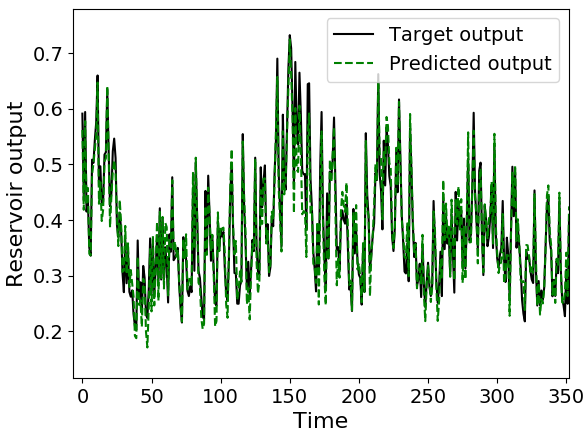
\includegraphics[width=2.5in]{img/narma_visualization.png}
  \caption{
    Visualization of reservoir output when fed the NARMA10 task. Input is an
i.i.d. stream generated uniformly in the interval [0, 0.5].
  }
  \label{visualization}
\end{figure}

\begin{figure}[H]
  \centering
  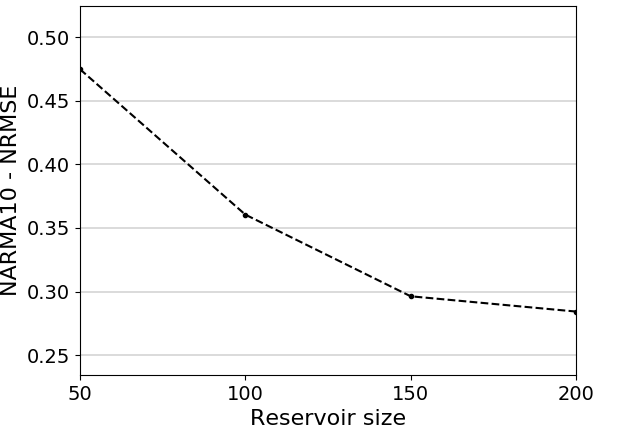
\includegraphics[width=2.5in]{img/general_performance.png}
  \caption{
    Reservoir size versus ESN performance for the NARMA10 task. The NRMSE is
averaged over 10 simulation runs.
  }
  \label{performance}
\end{figure}

All further reservoirs were constructed with the parameters from this baseline:
$\mathbf{W}^{res}$ and $\mathbf{W}^{in}$ were both generated as random matrices
with i.i.d. entries in the interval [-0.5, 0.5]. Both matrices are fully
connected, and the reservoir weight matrix was rescaled to have a spectral
radius of 0.9.

% (TODO): w_res density was also set to 0.2.

\subsection{Noise}

Key point: as long as we train with noise, we become more robust.

\begin{figure}[H]
  \centering
  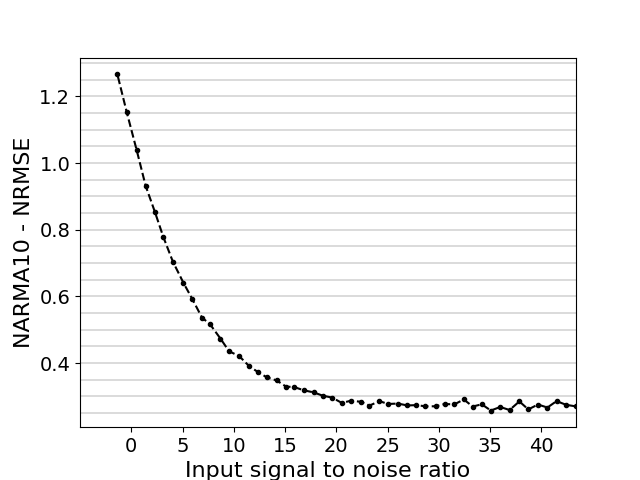
\includegraphics[width=2.5in]{img/input_noise_snr.png}
  \caption{
    Input noise SNR versus NRMSE.
  }
  \label{input_noise_snr}
\end{figure}

Some text.

\begin{figure}[H]
  \centering
  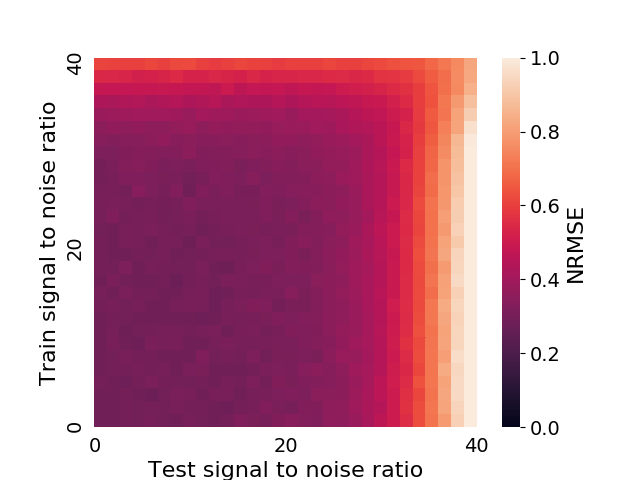
\includegraphics[width=2.5in]{img/input_noise_heatmap.png}
  \caption{
    Input noise signal to noise ratio for test/train.
  }
  \label{input_noise_heatmap}
\end{figure}

More text.

\subsection{Measurement equipment accuracy}

Text.

\begin{figure}[H]
  \centering
  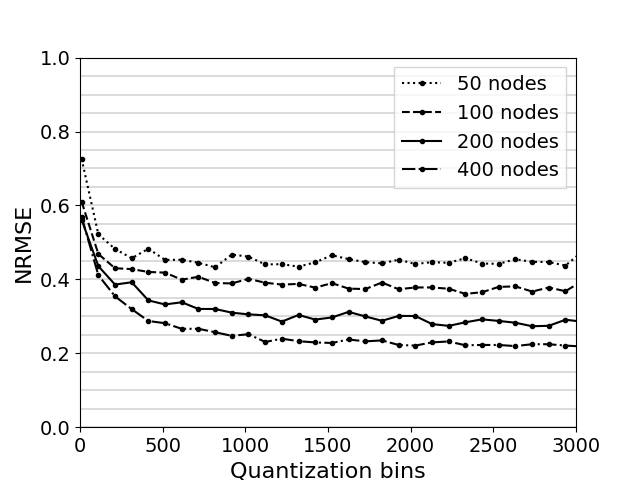
\includegraphics[width=2.5in]{img/adc_quantization.png}
  \caption{
    ADC quantization.
  }
  \label{adc_quantization}
\end{figure}

Text.

% Sensor anomalies, noise, amplifier gain and offset, ADC quantization (resolution
% error). The input analog voltage range is partitioned into a discrete number of
% values that the converter can measure, which is the ADCs resolution. How many
% steps would one have for a 12-bit ADC -- this should have very little meaningful
% impact on ESN performance?

\subsection{Partially visible state}

\begin{figure}[H]
  \centering
  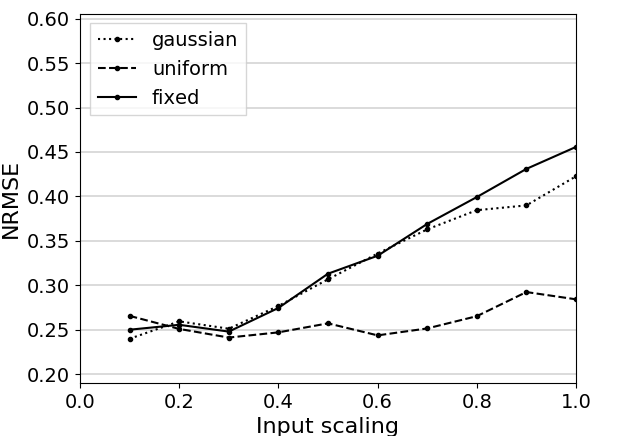
\includegraphics[width=2.5in]{img/input_scaling_distrib.png}
  \caption{
    Effect of input scaling on three input weight distributions.
  }
  \label{input_scaling_distrib}
\end{figure}

\begin{figure*}[htbp]
  \centering
  \begin{subfigure}{.3\textwidth}
    \centering
    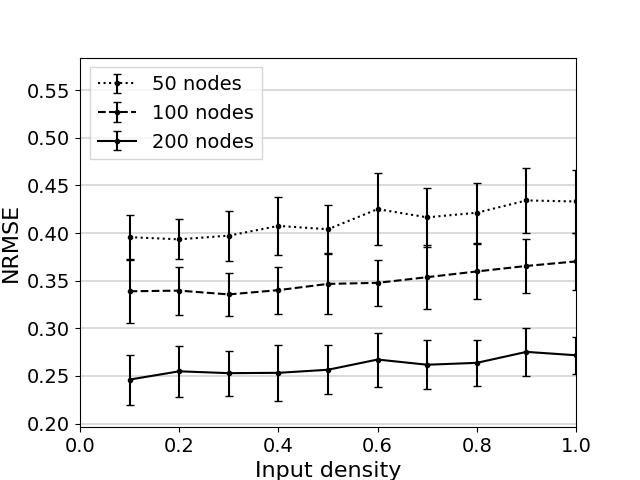
\includegraphics[width=\linewidth]{img/input_density_all.png}
  \end{subfigure}
  \begin{subfigure}{.3\textwidth}
    \centering
    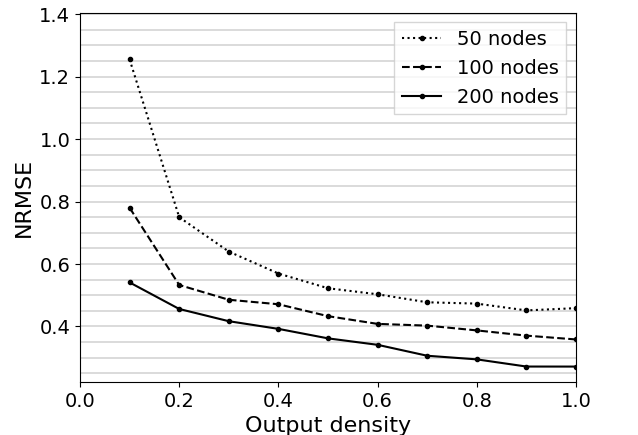
\includegraphics[width=\linewidth]{img/output_density_all.png}
  \end{subfigure}
  \begin{subfigure}{.3\textwidth}
    \centering
    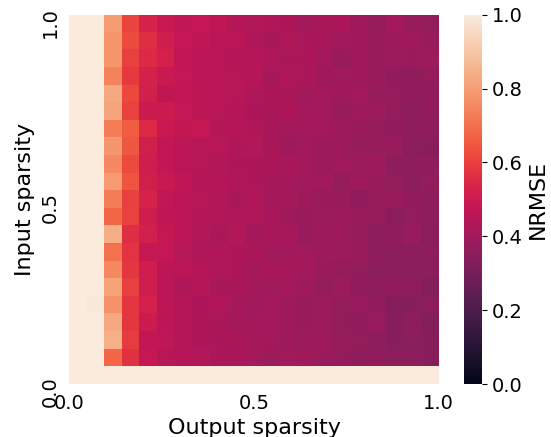
\includegraphics[width=\linewidth]{img/partial_visibility.png}
  \end{subfigure}
  \caption{
    These figures show the influence of reservoirs that are only partially
visible on the performance for the NARMA10 task. Experiments for the rightmost
plot were conducted using a reservoir size of 200 hidden nodes. The density is a
measurement for the fraction of elements in the input and output matrices
containing non-zero elements.
  }
  \label{partial_visibility}
\end{figure*}

% (TODO): Tie this together with topology, if it has a feed-forward-like structure
% or similar.

\subsection{Topology}

\begin{figure}[H]
  \centering
  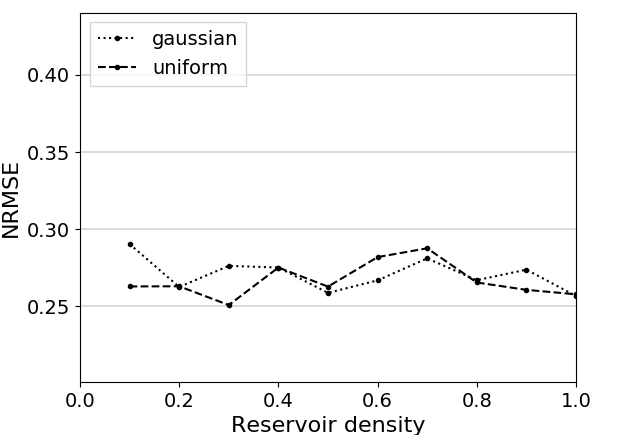
\includegraphics[width=2.5in]{img/reservoir_density_distrib.png}
  \caption{
    Reservoir density versus for two weight distributions. Fixed weight will not
work for internal nodes, unless special topology is employed, e.g. ring
(elaborate). This shows that sparse internal weight matrices work fine.
  }
  \label{reservoir_density_distrib}
\end{figure}

% (TODO): Is w_density also interesting for physical reservoirs?

%%% Local Variables:
%%% mode: latex
%%% TeX-master: "../main"
%%% End:
